\subsection{原型模式(Prototype)}

\subsubsection{原型模式简介}

原型模式是一种创建型设计模式,它的目的是通过复制一个已经存在的对象来创建新的对象,从而减少创建新对象的开销。原型模式通常适用于创建重复次数较多的对象,例如创建大量相同或相似的对象。

要实现原型模式,一般需要实现一个接口或抽象类,该接口或抽象类包含一个clone方法,用于复制当前对象。然后,需要创建一个具体的原型类来实现这个接口或抽象类,并在其clone方法中实现对象的复制。

原型模式有一些优点:

通过复制已经存在的对象,可以避免重新创建对象的开销,提高了效率。
可以通过改变复制出来的对象的属性值来实现对象的定制化,满足了开发者的个性化需求。
但是,原型模式也有一些缺点:

在实现原型模式时,需要实现一个接口或抽象类,这增加了系统的复杂度。

在Java中实现原型模式还需要实现Cloneable接口,并重写clone方法。由于Java语言中的clone方法是一个比较复杂的方法,它涉及到对象的浅复制和深复制,所以在使用时需要注意这些细节。

通常,原型模式适用于创建重复次数较多的对象,例如创建大量相同或相似的对象。例如,在游戏开发中,如果需要创建大量的游戏元素,比如怪物、道具等,那么可以使用原型模式来实现这些对象的快速创建。

此外,在项目开发中,如果需要从一个已经存在的对象中创建新对象,并且希望新对象具有与已经存在的对象相似的结构和功能,那么也可以考虑使用原型模式来实现这个功能。

总的来说,原型模式是一种非常有用的设计模式,它可以通过复制已经存在的对象来实现快速创建新对象的功能。在实际开发中,应根据实际情况来判断是否使用原型模式。

\subsubsection{原型模式在项目中的应用}

\begin{figure}[htb]
    \centering
    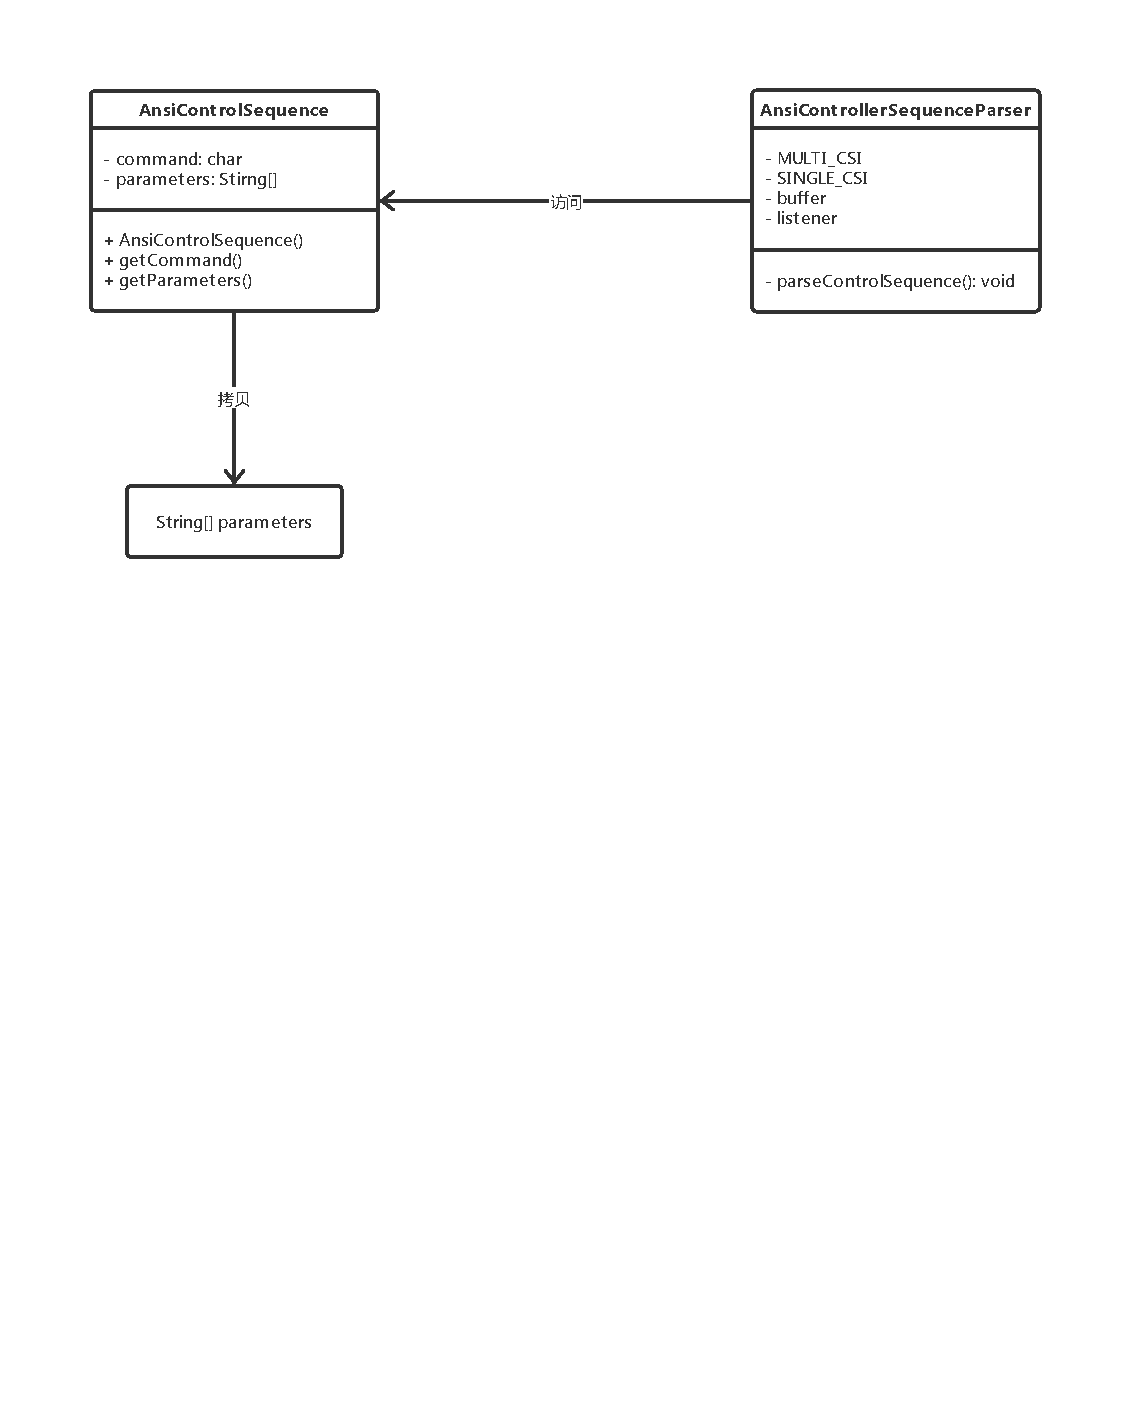
\includegraphics[width=0.9\textwidth]{figures/原型模式.pdf}
    \caption{原型模式在 Slow6502 中的类图}
\end{figure}

